\chapter{Hardware Accelerated Physics Simulation Frameworks}
\label{chp:back_PhysicsSimulators}


Testing control architectures directly on a physical robot often involves potential safety issues and prohibitive costs, which is why simulators play a major role in most robotics scenarios. As a matter of fact, especially when dealing with reinforcement learning as in the case study tackled in this work, the trial-and-error process needed for the agent to gain experience regarding the world may involve damaging complex and expensive hardware, limiting the possibility for the agent to explore and learn more efficiently. With the use of scalable physics simulators, there is the possibility of creating highly complex, customized environments to reproduce multiple scenarios, allowing also to have a testing environment that is as close as possible to the real world.

The most common way to speed up computations when simulating physical systems is to use hardware accelerators. In fact, the natural efficiency of \textit{Graphical Processing Units} and \textit{Tensor Processing Units} in solving parallel calculations can be exploited to cut down simulation times \citep{liang_gpu-accelerated_2018}. This is because the simulation can be approached as a set of independent tasks that can be executed at the same time diving the job among different cores. Although the use of \ac{GPU}s is the preferred choice for hardware accelerations, that requires in most cases writing low-level code in \ac{CUDA}, \cpp, or other low-level languages. This is not always the most immediate choice for rapid prototyping as it requires a lot of time to be spent on implementation, debugging, and final code polishing. Moreover, the use of low-level languages often leads to less readable code, which is not always the best choice when it comes to sharing the code with other researchers or developers, that is why the use of high-level languages like Python is often preferred.

At the time, the main physic simulation frameworks used for this purpose which have a Python accessible interface are Gazebo\footnote{\url{https://gazebosim.org}} \citep{koenig_design_2004} and Open Dynamics Engine, or ODE\footnote{\url{https://www.ode.org}}\citep{smith_open_2008} \citep{erez_simulation_2015,ivaldi_tools_2014}, thus if we restrict to the one used for reinforcement learning, \texttt{pybullet}\footnote{\url{https://pybullet.org}}\citep{coumans_pybullet_2016} and \texttt{mujoco}\footnote{\url{https://mujoco.org}}\citep{todorov_mujoco_2012} and Drake\footnote{\url{https://drake.mit.edu}}
\citep{tedrake_drake_2016}, are the most commonly used. Nevertheless, the former and the latter are not hardware accelerated. Moreover, neither of them offers a high-level interface to easily create complex environments, which is often the case when it comes to robotics research.
Regarding simulators that exploit hardware accelerations, NVIDIA \textsc{Isaac gym}\footnote{\url{https://developer.nvidia.com/isaac-gym}} \citep{makoviychuk_isaac_2021}, \texttt{brax} \citep{freeman_brax_2021} and most recently the \jax empowered MuJoCo XLA\footnote{\url{https://github.com/google-deepmind/mujoco/tree/main/mjx}} (MJX) are becoming the most popular choices.

\begin{figure}
    \centering
    \caption[MuJoCo Simulator GUI]{MuJoco Simulator \ac{GUI}.}
    \label{fig:mujoco}
    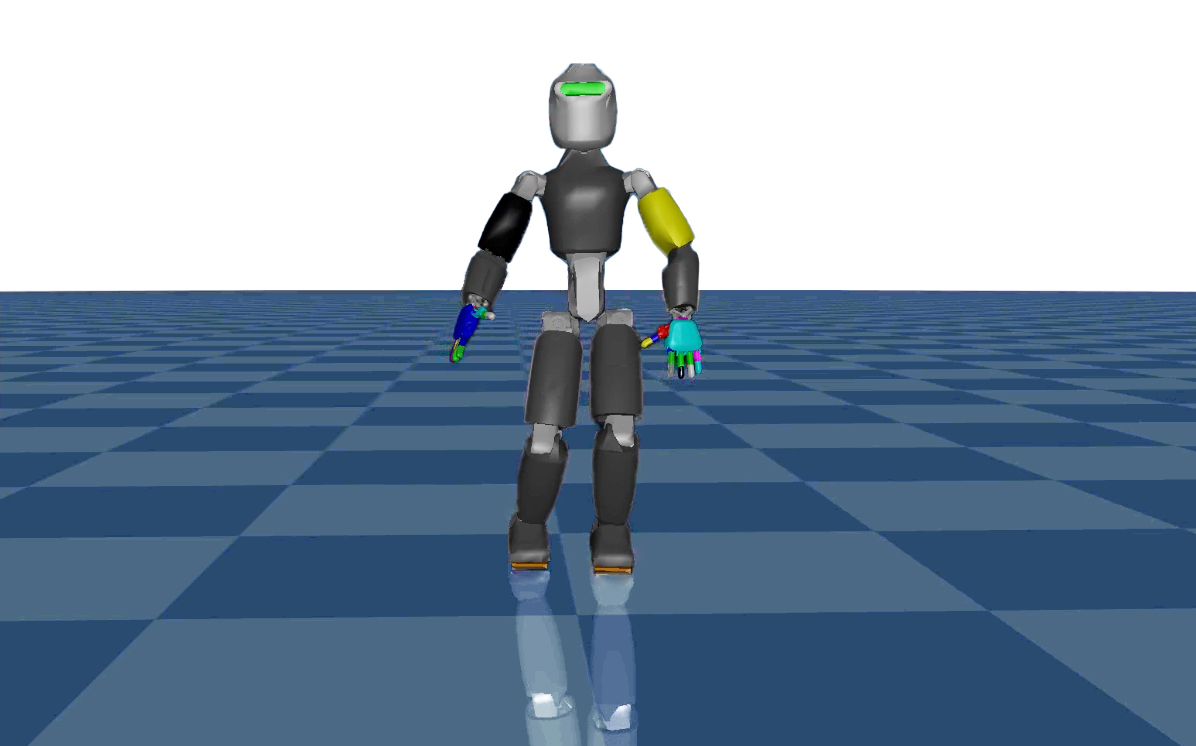
\includegraphics[width=0.7\textwidth]{Images/mujoco_ergocub.png}
\end{figure}

As robotics and reinforcement learning continue to merge and advance, with the increase of the environment and agent complexity, the computational cost of the simulation process increases as well, hence there's a growing demand for fast simulation environments that closely mimic real-world conditions. This is why these frameworks have a great impact on researchers, engineers, and developers to create and experiment with highly complex and realistic environments for training and testing \ac{RL} agents, essential for refining the control and decision-making capabilities of robots safely and efficiently. In the following sections, the physics simulators exploited in this work will be presented, highlighting their main features and limitations, with a focus on the implementation details of \jax, which is the core of the simulator used in the codesign loop.

\section{Nvidia ISAAC Gym}

\begin{figure}
    \centering
    \caption{NVIDIA Isaac Gym. (CHANGE)}
    \label{fig:isaac_gym}
    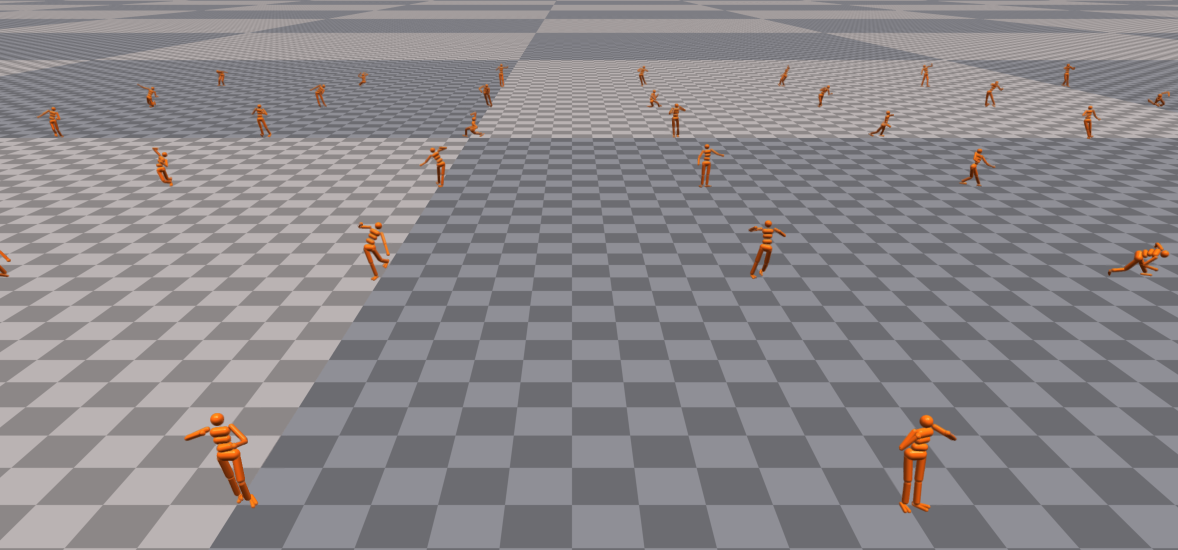
\includegraphics[width=0.7\textwidth]{Images/isaacgym_humanoid.png}
\end{figure}

In recent times, the use of \textit{Adversarial Motion Priors} \citep{peng_amp_2021} for reinforcement learning, which will be further discussed in \cref{chp:back_RLGA} has brought to the development of a new framework for physics simulation, called \textsc{isaac gym} \citep{makoviychuk_isaac_2021} which allows to simulate complex environments basing on \textsc{isaac sim} \citep{zhou_towards_2023}, a cyber-physical simulator that exploits NVIDIA PhysX and Omniverse, which offer a high-performance, cross-platform, real-time physics engine that allows to simulate rigid bodies in reduced coordinate articulations. \textsc{Isaac gym} then leverages the power of \texttt{rl\_games} \citep{rl-games2021} to completely work with \texttt{pytorch} \citep{paszke_pytorch_2019} tensors on \ac{GPU}s to accelerate the simulation process, allowing to train complex environments with multiple agents and objects.

The backend implementation of the simulator is written in \cpp while offering a frontend interface in Python, which allows us to easily build complex environments and agents, as well as to visualize the simulation process. Nevertheless, being the framework completely closed-source, it is not possible to extend the functionalities of the simulator, which is limited to the ones provided by the original developers.

\section{JAX: High-Performance Array Computing}

\begin{figure}
    \centering
    \caption{JAX Overview.}
    \label{fig:jax_logo}
    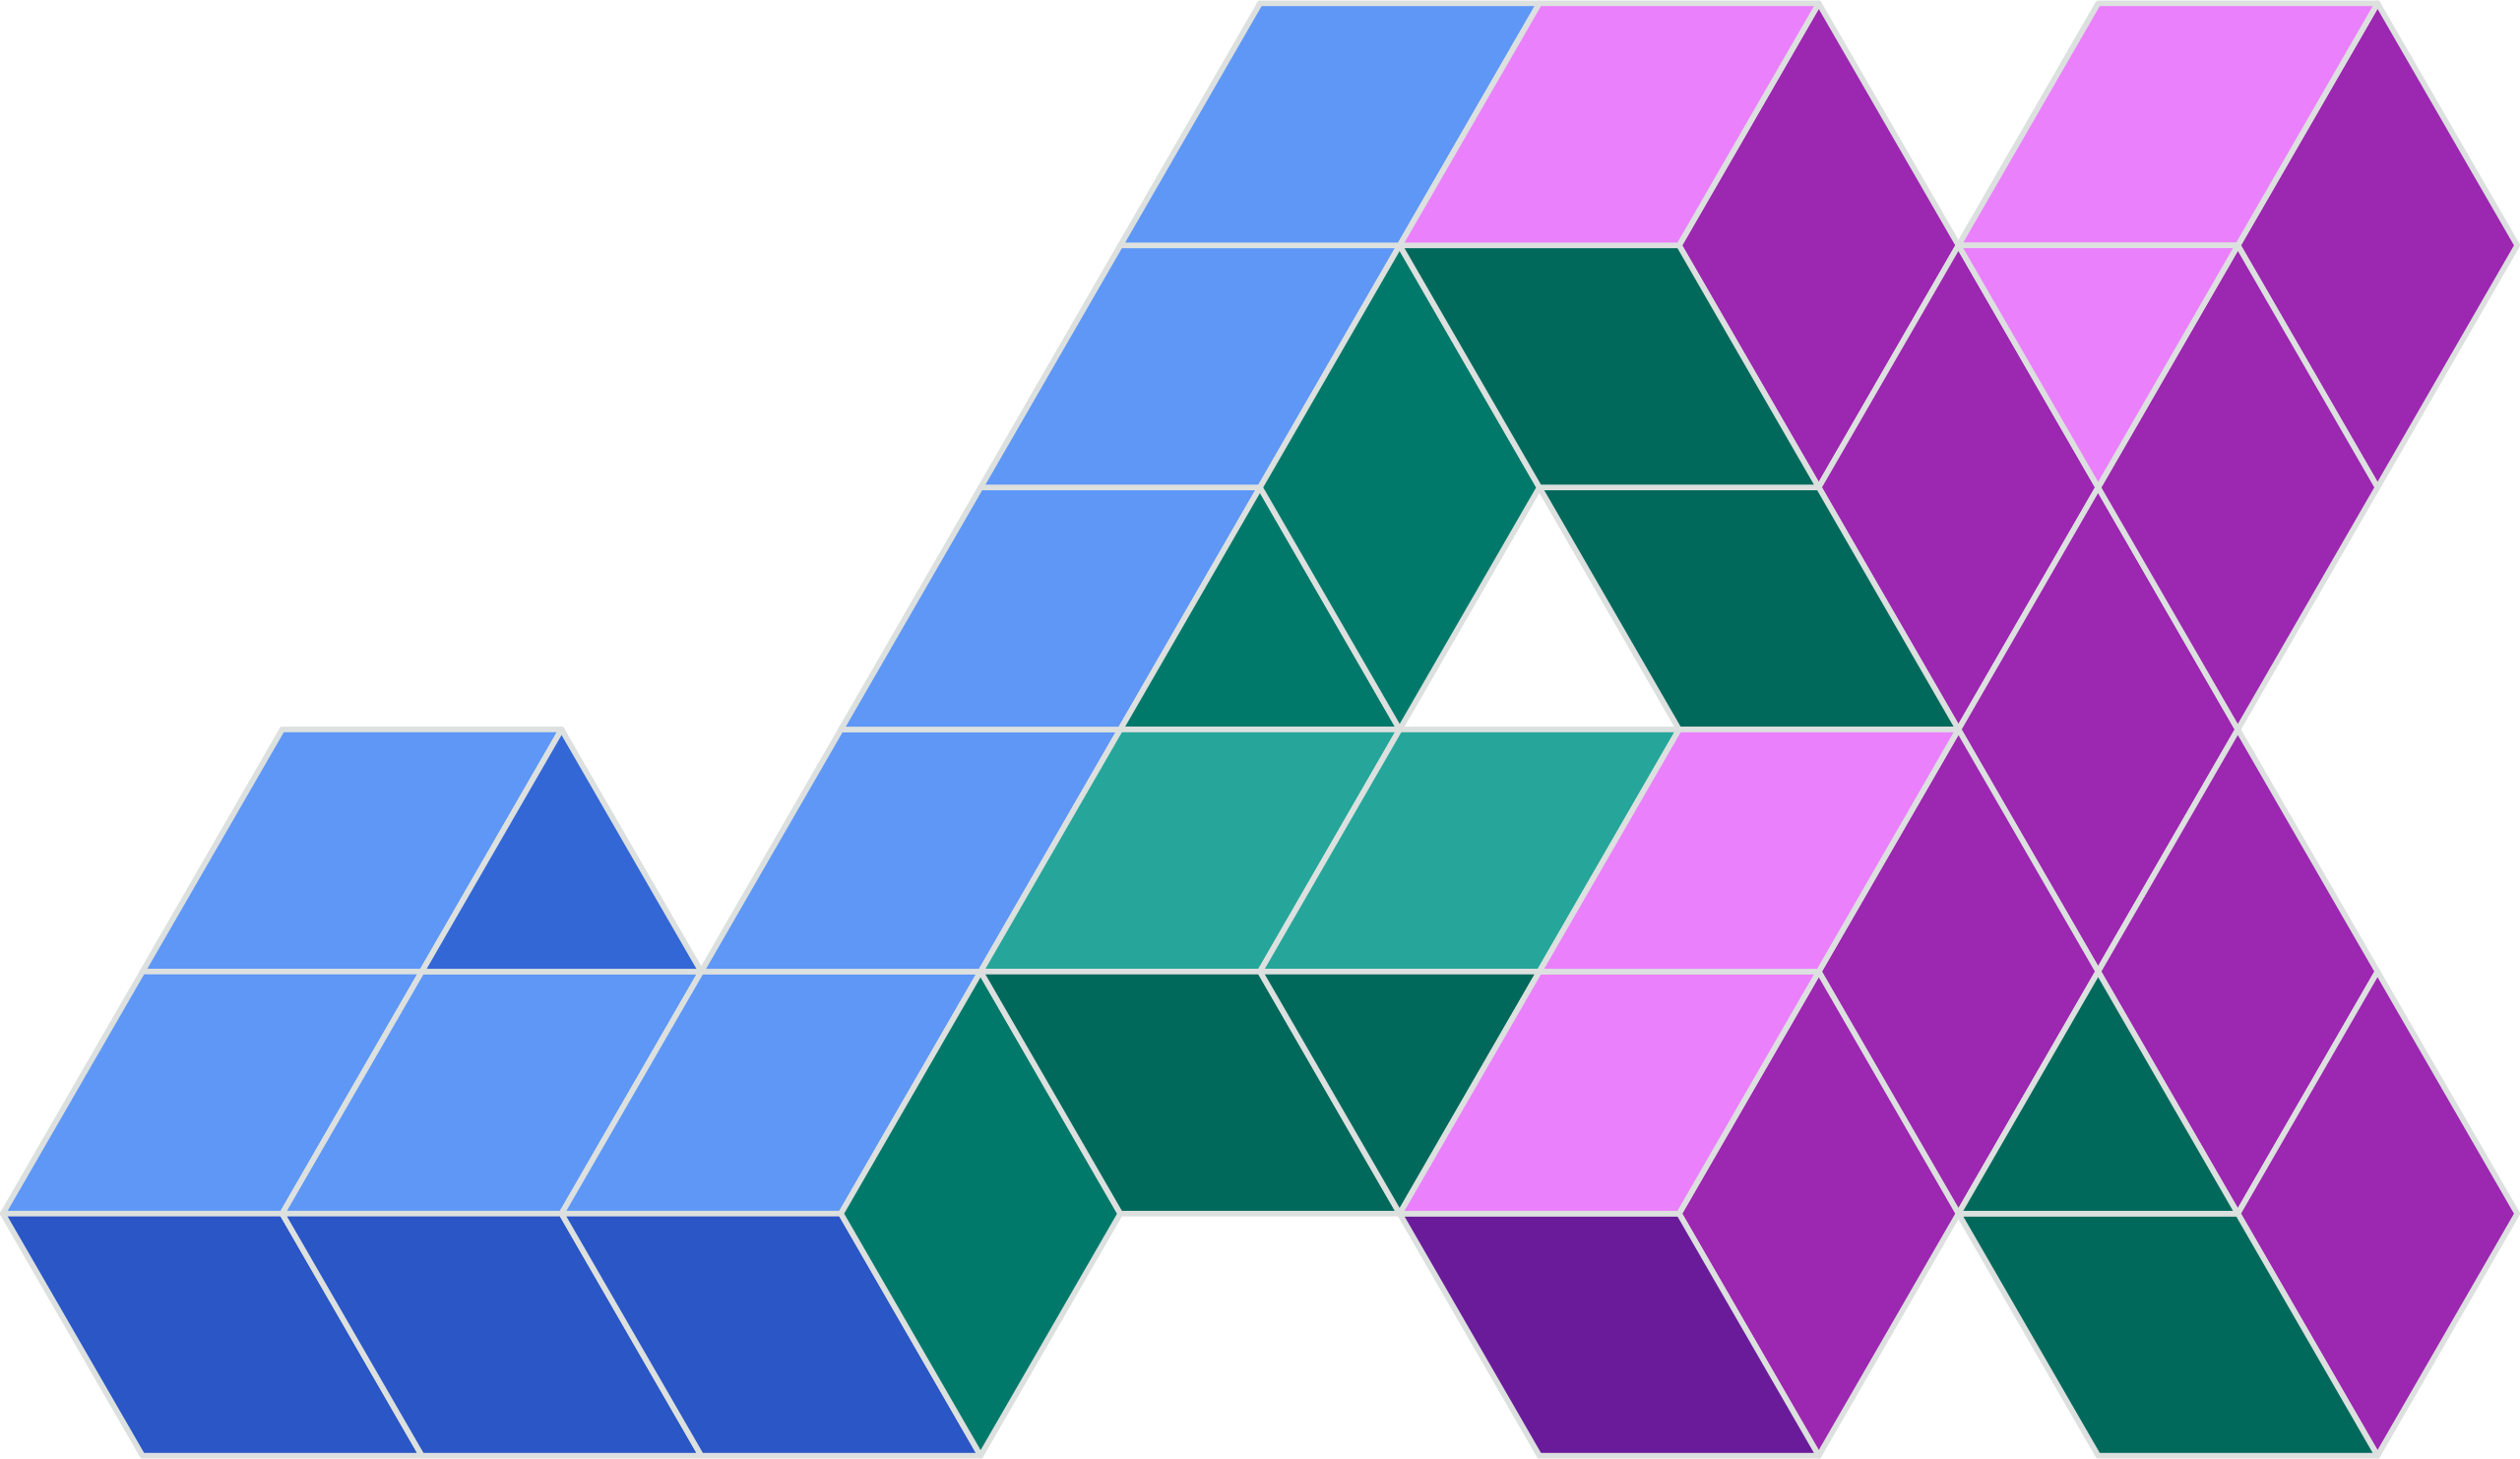
\includegraphics[width=0.3\textwidth]{Images/jax_logo.png} \qquad \qquad
    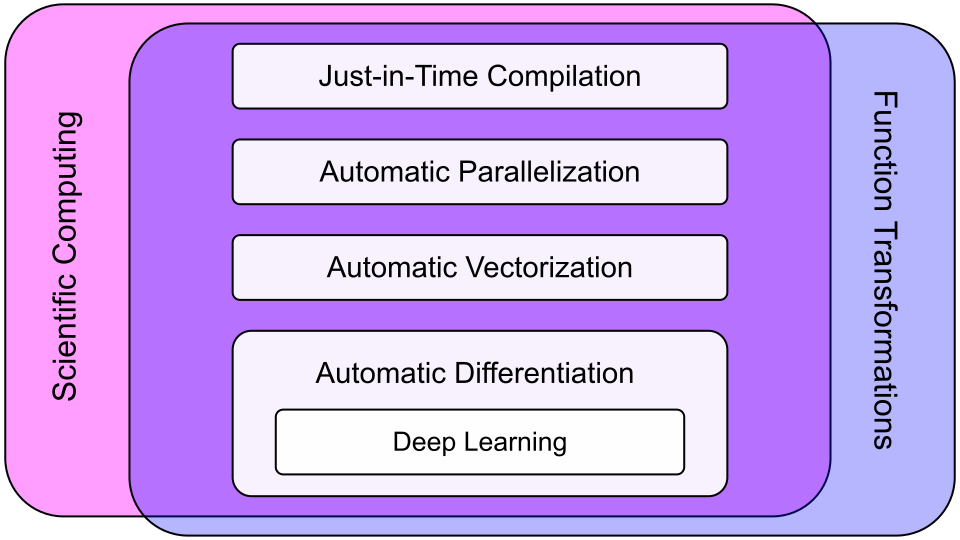
\includegraphics[width=0.4\textwidth]{Images/JAX-overview.png}
\end{figure}

Amongst the variety of framework that offers a high-level interface to make it easier for the user to write code that can be run on \ac{GPU}s, \jax \footnote{\url{https://github.com/google/jax}} \citep{bradbury_jax_2018,47008} is rapidly becoming one of the most popular choices. It exploits the power of \ac{XLA} \citep{50530}, which is a domain-specific, \textit{Just-In-Time} (\ac{JIT}), graph-based compiler for linear algebra that leverages efficient kernel fusion and lazy tensor materialization, firstly developed for TensorFlow \citep{tensorflow2015-whitepaper} and then extended to PyTorch and \jax itself.
Computations on \textit{Central Processing Units} (\ac{CPU}) also benefit from the use of \ac{JIT} compilation and fused operations \citep{wang_kernel_2010,snider_operator_2023}. \ac{JIT} compilation allows to compile the code at runtime, while fused operations combine multiple algebraic operations into a single \textit{Fused Multiply-Add} operation(\ac{FMA}), reducing the overhead of the compilation process and avoiding intermediate results by rounding the result of the multiplication to the nearest representable number in the given precision.
Moreover, \jax supports back and forward \textit{Automatic Differentiation} (\ac{AD}), which is a key feature for the implementation of deep learning (DL) algorithms, physical system modeling, and optimization.

A fresh and interesting alternative to \jax, that allows one to easily write \ac{GPU}-accelerated Python code is NVIDIA Warp \citep{warp2022}, which uses a kernel-based programming model that triggers \ac{JIT} compilation of Python code. The compilation generates \textit{Parallel Thread Execution}s (\ac{PTX}) as an intermediate representation, which is then transformed into \textit{CUDA} code. With Omniverse integration, as a key feature, it supports the simulation of mesh grids, cloths, particles, and fluids, as well as the simulation of rigid bodies. Nevertheless, it is still in its early stages of development and it is not yet widely used in robotics research.


\subsection{JAX Implementation Details}

\jax uses a set of low-level primitives to support high-level array operations, which have the characteristic to be differentiable and \ac{JIT} compilable. What happens under the hood is that the Python callable gets traced, generating an \textit{Intermediate Representation} (\jax IR) which is a functional representation of the program. The \jax transformations like \texttt{vmap} and \texttt{grad} that allow vectorizing and differentiate the function, are then applied to the \jax IR, finally lowering to \ac{XLA} operations, ready to be executed on \ac{GPU} or \ac{TPU} devices.


\begin{figure}
    \centering
    \caption{JAX Tracing and Compilation Process.}
    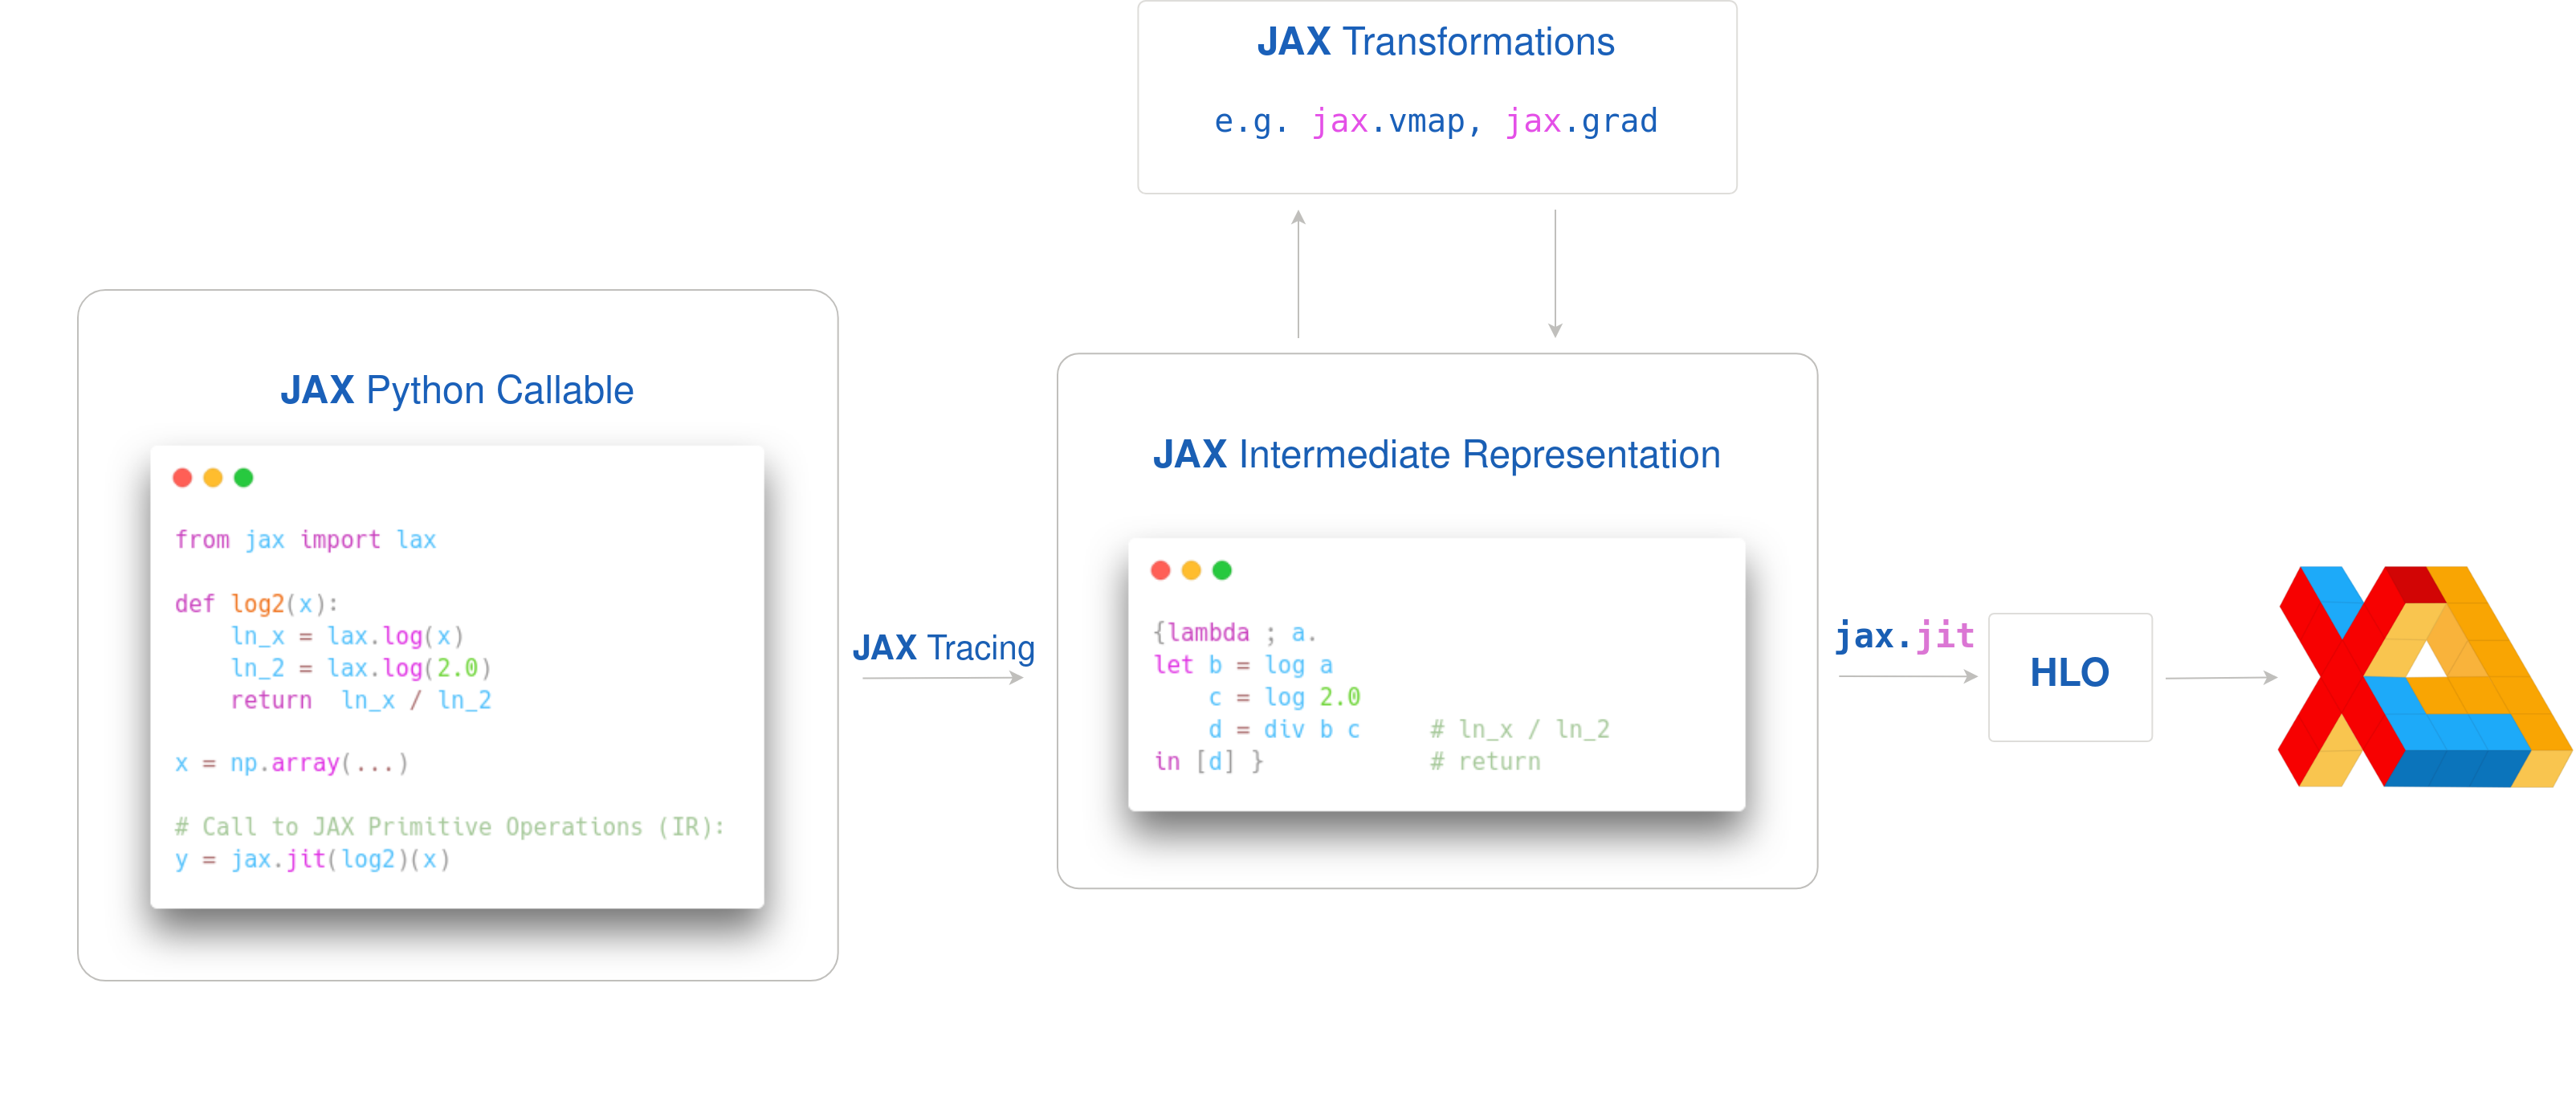
\includegraphics[width=\textwidth]{Images/jax_compute_graph_short.png}
\end{figure}

Creating \jax code requires following a set of rules ensuring that the code can be compiled and potentially auto-differentiated. In fact, \ac{JIT} compilation requires the code to have static bounds on memory requirements and statically-typed, which is not trivial in a dynamically-typed language as Python.
For example, the usage of \texttt{for}-loops and \texttt{if}-statements is not so straightforward, as the former involves dynamic iteration, which can disrupt the static nature of the code and will get unrolled during the compilation process, leading to a potentially huge computation graph causing memory issues, long compilation times and the impossibility to be forward and backward differentiated. The latter instead introduces conditional branches in the computation graph which cannot be managed by the \ac{XLA} compiler in a static way at runtime. Nevertheless, \jax offers a set of functions that allows to perform static iteration and conditional branching while being forward and backward differentiable and automatically compiled in \textit{Just-In-Time}, namely, \texttt{jax.lax.scan} and \texttt{jax.lax.cond}. Similarly, \texttt{while}-loops do not support reverse differentiation, but they can be implemented using \texttt{jax.lax.scan}, in which the termination condition is checked at each iteration, and when it is met, the loop is not stopped, but the iteration simply does not update the state, ensuring that the number of iterations is static and known at compile time.

\begin{figure}
    \centering
    \caption{JAX vs Native Python For Loop.}
    \label{fig:jax_python_forloop}
    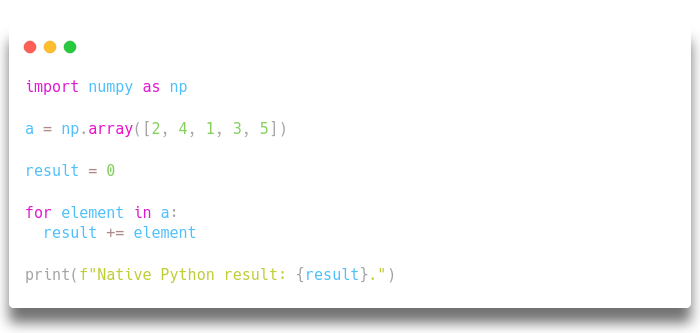
\includegraphics[width=0.45\textwidth]{Images/python_forloop.png}
    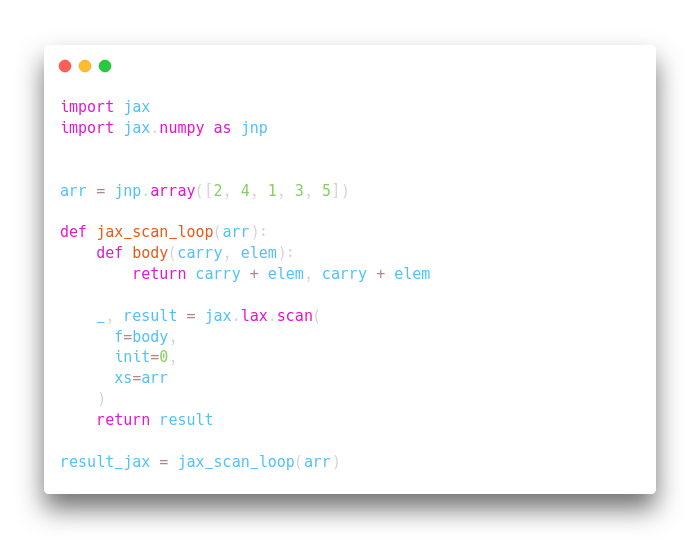
\includegraphics[width=0.45\textwidth]{Images/jax_forloop.png}
\end{figure}

Using \texttt{jax.lax.scan} and \texttt{jax.lax.cond} requires writing the code in a functional programming style, which is not always the most immediate choice for the user. In the examples reported in \cref{fig:jax_python_forloop}, a \texttt{body} function will get executed at each iteration which will have an initial value for the variable \texttt{carry} of \texttt{0} and will iterate through \texttt{arr}. The \texttt{cond} function will instead execute the \texttt{true\_fun} function if the condition \texttt{cond} is met, otherwise, it will execute the \texttt{false\_fun} function, as reported in \cref{fig:jax_python_if}. Note that with respect to the Python implementation, the \jax implementation requires declaring the type of the variable \texttt{x} as a \texttt{jax.numpy.ndarray}, this will ensure the creation of a \textit{PyTree} object.

\begin{figure}
    \centering
    \caption{JAX vs Native Python If Statement.}
    \label{fig:jax_python_if}
    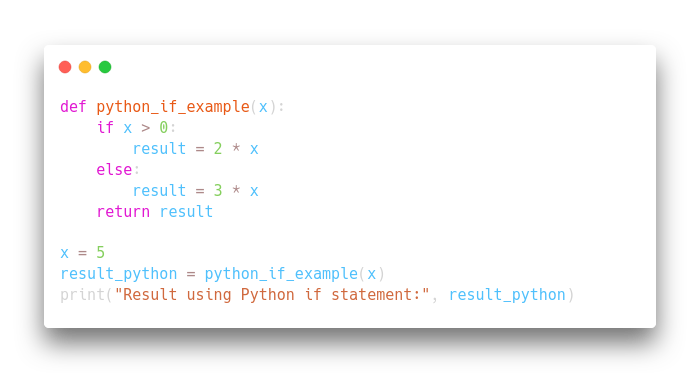
\includegraphics[width=0.49\textwidth]{Images/python_if.png}
    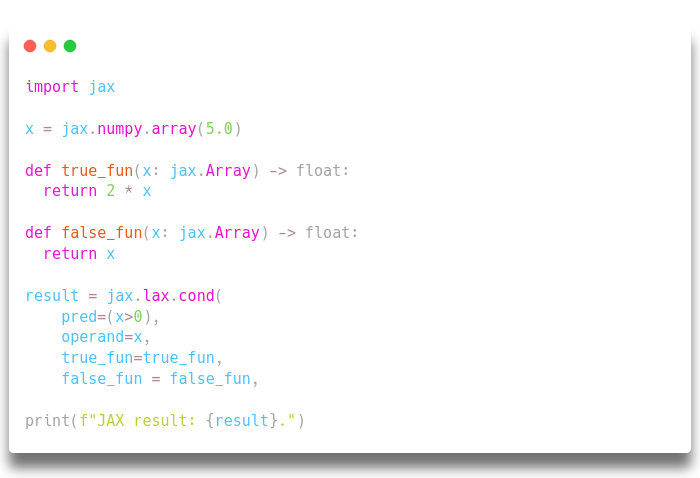
\includegraphics[width=0.49\textwidth]{Images/jax_if.png}
\end{figure}

Furthermore, \jax introduces a new optimized structure for convenient simple operation on heterogeneous data structures, called \textit{PyTree}s, which is an object with a tree-like structure that can be used to represent nested data structures. The main advantage of using \textit{PyTree}s is that they can be used to represent and perform operations on heterogeneous data structures. In the example shown in \cref{fig:pytree_example} in fact, the \texttt{pytree} variable is an object containing four different data structures, thus being the \textit{leaves}, i.e. the outermost elements of the tree, compatible among each other, by calling \texttt{jax.tree\_map} on the \texttt{pytree} object, the function \texttt{x+1} can be applied to each leaf of the tree, returning a new \textit{PyTree} object with the same structure of the original one, but with the leaves modified by the function.

\begin{figure}
    \centering
    \caption{Example Operation on a JAX PyTree.}
    \label{fig:pytree_example}
    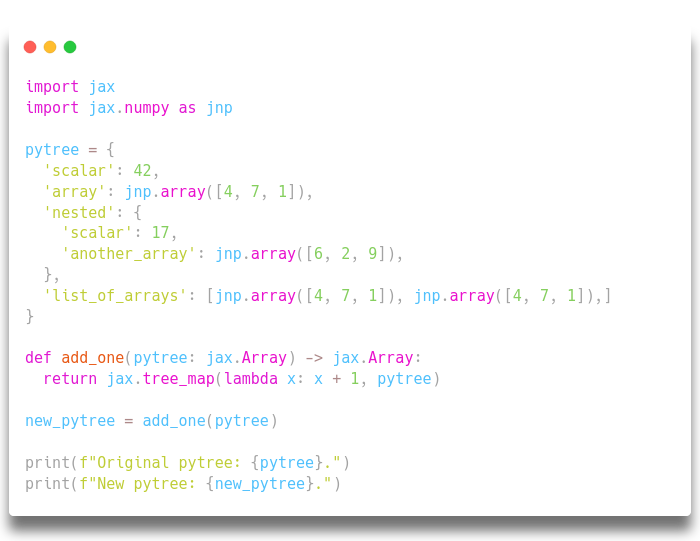
\includegraphics[width=\textwidth]{Images/pytree_example.png}
\end{figure}

\section{JAXsim}

It is immediate to think of the possibility of combining the power of \jax with the flexibility and ease of use of Python to create a physics simulator that can be easily extended and customized. This was the main idea behind \texttt{brax} \footnote{\url{https://github.com/google/brax}} \citep{freeman_brax_2021}, a differentiable rigid body physics simulator in maximal with the most recent $v2$ release, reduced coordinates. Nevertheless, the absence of a high-level interface to immediately get the mechanical system quantities of the Euler-Poincare equation, as well as the lack of support for \ac{SDF} files, often used in model-based robotics research, led to the development of \jaxsim \footnote{\url{https://github.com/ami-iit/jaxsim}} \citep{ferigo_jaxsim_2022}, a hardware-accelerated physics simulator that exploits the strong parallelization capabilities and the \ac{JIT} compilation of \jax to speed up the simulation process.

Although being functional programming preferable in \jax, \jaxsim makes use of \textit{Object Oriented Programming} (\ac{OOP}) in order to create a modular and extensible framework easily accessible to the user. At this scope, the static nature of the objects is ensured throughout the simulator by using frozen \texttt{dataclasses}, which are immutable objects that cannot be modified after their initialization unless their mutability gets explicitly set, thus ensuring that the \textit{PyTree} structure of the objects is preserved when performing operations on them via the usage of context managers.

The use of \ac{OOP} is exploited in this work in order to add a layer of abstraction to the simulator, which allows to easily simulate the dynamics of motors inside the joints of a robotic system while maintaining the same interface of the original \jaxsim framework.


\section{Impacts and Contacts}
\label{sec:back_contacts}

When dealing with rigid body dynamics, the most common approach to model the contact between two bodies is to use a \textit{penalty-based} approach \citep{inproceedings}, which consists of adding a force to the system when the distance between two bodies is below a certain threshold. This approach is computationally efficient and easy to implement, but it does not allow to model the dynamics of the contact, which is often the case when dealing with high-velocity impacts. In fact, in the case of a high-velocity impact, the contact between two bodies is not perfectly inelastic, hence the partial elasticities of the materials involved in the collision induce vibrational modes in the system. This is why a \textit{compliant} approach is often preferred, which allows to model the dynamics of the contact, but it is computationally more expensive and requires a more complex implementation.

\subsection{Smooth Impacts}

In a high incident velocity impact between two solids, due to the nonperfect inelasticity, some of the kinetic energy is transferred to the vibrational model.

Considering a point particle with mass $m$ and position $\mathbf{p}(t): \mathbb{R} \rightarrow \mathbb{R}$ in a one-dimensional space, compliant with a spring with stiffness $k$ and a damper with damping coefficient $c$, the resulting force generated can be defined as:

\begin{equation}
    F = \begin{cases}
        -k\mathbf{p} - cv & \text{if } \mathbf{p} > 0    \\
        0                 & \text{if } \mathbf{p} \leq 0
    \end{cases}
\end{equation}

Considering an initial position $\mathbf{p}(t=0) = 0$ and a starting velocity $v_0 \in \mathbb{R}$ such that $v(t=0) = v_0 > 0$, i.e. the particle starts at the origin but moves towards the penetration region, will result in an active force $F(t) = -k\mathbf{p}(t) - cv(t)$ that will be applied to the particle until it reaches the equilibrium position $\mathbf{p} = 0$. The resulting motion will be a damped oscillation that can be derived from the Lagrangian mechanics as seen in \cref{eqn:lagrangian}, where the Lagrangian $\mathcal{L}$ of the system is defined as:

\begin{equation}
    \mathcal{L} = \mathcal{T} - \mathcal{V} = \frac{1}{2}mv^2 - \frac{1}{2}k\mathbf{p}^2
\end{equation}

which yields the following equation of motion:

\begin{equation}
    \ddot{\mathbf{p}} + \underbrace{\frac{c}{m}} _{\omega ^2} v + \underbrace{\frac{k}{m}} _\gamma \mathbf{p} = 0 \quad \rightarrow \quad \ddot{\mathbf{p}} + 2\zeta \omega v + \omega ^2 \mathbf{p} = 0
\end{equation}

where $\omega$ is the natural frequency of the system and $\gamma$ can be used to declare the damping ratio $\zeta = \frac{\gamma}{2\omega}$.

The solution of the resulting equation is the one of a first-order linear \ac{ODE}:

\begin{equation}
    \mathbf{p}(t) = \mathbf{p}_0 e^{-\zeta \omega t} \cos(\omega \sqrt{1 - \zeta ^2} t)
\end{equation}

which implies an oscillatory regime for $\zeta < 1$ and an exponential decay for $\zeta > 1$, also called overdamped regime.
Although relatively simple to implement, this approach is not always the most efficient, as it requires solving a \textit{differential algebraic equation} at each time step, which can be computationally expensive, making it extremely sensitive to the choice of the time step $h$.

\subsection{Non-smooth Impacts}

Considering two bodies and given the surface points $p ^{(0)}$ fixed on body 0 and $p ^{(1)}$ fixed on body 1, the \textit{signed} distance between the two should be non-negative i.e. $c(p ^{(0)}, p ^{(1)}) \geq 0$, in order to avoid comprenetration.

The impact involves forces that change rapidly to cause jump discontinuities in the velocities $\dot{q}$. Therefore it is possible to state that the velocity before and after the impact at time $t_i$ differ:

\begin{equation}
    \lim _{t \uparrow t _i} \dot{q} = \dot{q} _{-} \neq \dot{q} _{+} = \lim _{t \downarrow t _i} \dot{q}
\end{equation}

Mathematically, the position $q(t)$ remains continuous while the velocity $\dot{q}(t)$ exhibits jump discontinuities, hence the acceleration $\ddot{q}(t)$ is not defined at impact times.

Considering the case of a spherical rigid body impacting an infinite plane, the convexity of the two objects implies that the closest point between the two can be identified uniquely. By writing the signed distance function with respect to the rigid body center of mass position $x(t)$, we get that $c(q(t)) = \tilde{c}(x(t)) \geq 0$, yet when the sphere is in contact with the plane we have that $\tilde{c}(x(t)) = 0$. With this approach, we can define two configuration manifolds: $Q _1 \subset \mathbb{R} ^2 \times \mathrm{SO}3$ for the planar motion and $Q _2 \subset \mathbb{R} ^3 \times \mathrm{SO}3$ for the spatial motion. Without loss of generality, the problem can be simplified in notation by defining a Lagrangian multiplier $\xi \in \mathbb{R}$ corresponding to the magnitude of the force acting in the normal direction at the contact point while keeping a configuration manifold $Q \in \mathbb{R}^3 \times \mathrm{SO}(3)$.
By using the augmented Lagrangian, the \cref{eqn:lagrangian} can be rewritten as:

\begin{equation}
    \frac{d}{dt} \frac{\partial}{\partial \dot{q}} \mathcal{L} - \frac{\partial}{\partial q} \mathcal{L} - J^\top \lambda = 0 \quad \text{and} \quad \varepsilon\lambda + g(q) = 0
\end{equation}

where $\lambda$ are the coordinates of $m$ one-dimensional point particles having position $\lambda _{j}$, $J$ is the Jacobian and  $g \in Q \times \mathbb{R} \rightarrow \mathbb{R} ^m$ is the configuration coordinate function, and by discretizing the time with a fixed time step $h$, we get:

\begin{equation}
    \int _0 ^h ds\xi^\top c(q(s)) \sim h\xi_0 ^\top c_0
\end{equation}

as the least action principle requires the discrete action to be minimized over the allowed trajectories $c(q_k) >0$, using the theorem of Karush-Kuhn-Tucker, we get to a stationarity condition that does not allow for energy conservation \citep{lacoursiere_ghosts_2007}.

\subsection{Approximate Impulse Model}

In a discrete mechanics framework, defining $h$ the fixed time step for all steps, if the violation in the impact point at step $i$ called $q _i$ is not too big, a good approximation of the incident velocity is:

\begin{equation}
    \dot{q} _{-} = \frac{q _i - q _{i-1}}{h}
\end{equation}

To estimate the outbound velocity $\dot{q} _{+}$ instead, we impose the discrete impulsive Newton impact law in one spatial dimension as:

\begin{equation}
    \dot{q} _{+} = -\psi \dot{q} _{-}
\end{equation}

where $\psi \in [0,1]$ is the \textit{restitution coefficient}.

A perfectly elastic collision corresponds to $\psi = 1$ in which the outbound velocity is the reflection of the incoming one. Now, given that the impulse occurs at a fixed position $q$, the only change in energy is a kinetic energy change, hence for the Newton-Poisson impact law for a point particle of mass $m$ with kinetic energy $\mathcal{T}(q, \dot{q})$, the change in energy is:

\begin{equation}
    E _{+} - E _{-} = \mathcal{T}(q, \dot{q} _{+}) - \mathcal{T}(q, \dot{q} _{-}) = (\psi ^2 - 1) \mathcal{T}(q, \dot{q} _{-}) \leq 0
\end{equation}

To generalize in three dimensions, we define an estimate of the normal component of the incident velocity with respect to the contact manifold as $C _k \dot{q} _{-}$ where $C _k$ is the $n _c \times n$ Jacobian matrix of the $n _c$ contact surface evaluated at the discrete time $k$. Using the complementarity formulation, assuming the presence of other inequality constraints with the agglomerated Jacobian $J$, adding regularization parameters with diagonal non-negative matrices $\Sigma$ and $\Xi$, and considering the diagonal matrix for restitution coefficients $\Psi = \text{diag}(\psi _1, \psi _2, \dots, \psi _{n _c}),  \psi _i \in [0, 1]$, we get the following linear complementarity problem (LCP):

\begin{equation}
    \begin{rcases}
        M\dot{q} _{+} - G ^\top _k \lambda - C ^\top _k \dot{q} & = M \dot{q} _{-}    \\
        G _k \dot{q} _{+} + \Sigma \lambda                      & = G _k \dot{q} _{-} \\
        C _k \dot{q} _{+} + \Psi C \dot{q} _{-} + \Xi \dot{q}   & = w                 \\
    \end{rcases} \quad \text{subject to
        :  } \quad \dot{q} \geq 0 \perp w \geq 0
\end{equation}

By solving the optimization above, it can be shown that this leads to $T _{+} \leq T _{-}$, therefore the impulsive stage can only decrease the kinetic energy.
